\chapter{Introducción}
\label{cap:introduccion}

\chapterquote{Sólo hay una victoria decisiva: la última}{Carl Von Clausewitz}

El presente Trabajo de Fin de Grado aborda el diseño y la implementación de un motor de
exploración de colecciones digitales que combina filtrado facetado por metadatos, navegación
transversal entre colecciones relacionadas y operaciones de conjuntos sobre los resultados.
La propuesta nace en respuesta a un problema concreto del consumo de información digital
contemporáneo, que motivamos a continuación, y persigue devolver al usuario una herramienta
que combine la precisión de la búsqueda directa, la flexibilidad del filtrado por etiquetas y
la riqueza expresiva de la navegación hipermedia.

Este capítulo introductorio se organiza en tres bloques: la motivación que originó el trabajo,
los objetivos perseguidos y el plan de ejecución del proyecto.

\section{Motivación}
En los últimos tiempos hemos pasado por un gran cambio en el paradigma de consumo digital.
El acúmulo cuantitativo de contenidos digitales ha sobrepasado su umbral cualitativo y hoy supone una 
manera distinta de relacionarse con ello.
La abundancia de información genera una «sobrecarga de información» (o \textit{information overload}),
en la cual el usuario necesita una cantidad cada vez mayor de tiempo para navegar.
Esto se hace especialmente evidente en las plataformas digitales, en particular las de \textit{streaming} multimedia
(como Netflix, Disney+ y HBO Max), en las que difícilmente encontramos qué consumir sin invertir un tiempo sustancial
en ello.

Este cambio de paradigma, y el subsecuente problema, sigue siendo abordado con métodos tradicionales como la
búsqueda directa (por palabras clave), el filtrado clásico por género o medio y los sistemas de recomendación
basados en algoritmos ocultos al consumidor.
Estos enfoques son limitados y sirven poco al nuevo contexto de consumo digital.
La búsqueda directa es determinista y no permite flexibilidad alguna, ya que presupone que el usuario
sabe exactamente lo que está buscando de antemano.
El filtrado tradicional suele ser incompleto e inconsistente, al apoyarse en taxonomías ocultas e inescrutables.
Los algoritmos de recomendación suelen actuar más como propagadores de la burbuja de filtros
(o \textit{filter bubble}), al depender directamente del historial de consumo o de lo que la plataforma
desee promover, restando agencia al usuario en última instancia.

Este problema, sin embargo, no es exclusivo de la experiencia de usuario, sino que también supone un problema tecnológico
relacionado con la forma en la que se diseñan y utilizan las colecciones de información.
Los modelos relacionales de navegación y los sistemas de navegación sobre colecciones
(\textit{collection navigation systems}) plantean un enfoque distinto, en el que los datos no se
representan como elementos aislados, sino como entidades conectadas mediante relaciones semánticas.
Este enfoque permite recorrer colecciones de manera interactiva, con mecanismos de navegación más expresivos
en los que el usuario puede explorar progresivamente una colección compleja combinando filtros, relaciones y
transiciones entre entidades.

Existe, por lo tanto, una necesidad declarada de que los sistemas de navegación acompañen este cambio de paradigma.
Esto solo se puede satisfacer ofreciendo a los usuarios herramientas de exploración interactiva más ricas y flexibles.
Dichas herramientas deben combinar la precisión propia de la búsqueda directa con una expresividad mayor
que la del filtrado clásico, sin restar agencia al usuario.

\section{Objetivos}
\label{sec:objetivos}

El presente Trabajo de Fin de Grado parte de la propuesta original del profesor, titulada
\textit{Aplicación para el procesamiento de colecciones de contenidos digitales}, que planteaba
el diseño de una herramienta para transformar metadatos y contenidos de objetos en grandes
colecciones digitales, con posibilidades que iban desde la recodificación de descripciones hasta
el etiquetado asistido por modelos del lenguaje. A partir de esa propuesta inicial hemos
delimitado el alcance hacia la \textbf{exploración interactiva} de colecciones, conservando la
idea central de un sistema agnóstico al dominio capaz de operar sobre colecciones heterogéneas,
pero concentrando el esfuerzo en las primitivas de navegación que permitan al usuario recorrerlas
de forma expresiva. Esta acotación está sustentada por la naturaleza experimental del motor de
navegación que se quería validar y por el deseo de entregar un sistema funcionalmente cerrado al
término del trabajo; queda como línea de continuación natural, recogida más adelante entre las
líneas futuras, la integración de transformaciones asistidas por modelos del lenguaje sobre el
mismo motor.

\subsection*{Objetivo general}

Diseñar e implementar una aplicación de exploración interactiva de colecciones digitales que
combine filtrado facetado por metadatos, navegación transversal entre colecciones relacionadas
mediante referencias semánticas, y operaciones de conjuntos sobre los resultados parciales, todo
ello bajo un modelo de datos agnóstico al dominio que permita aplicar el sistema a colecciones
de naturaleza estructural distinta sin modificaciones sustanciales.

\subsection*{Objetivos específicos}

A partir de ese objetivo general identificamos seis objetivos específicos, formulados de manera
que puedan verificarse de forma independiente en el capítulo de Pruebas y Validación.

\begin{itemize}
\item \textbf{O1. Modelo de datos agnóstico al dominio.} Definir un modelo relacional que
represente colecciones, entidades, metadatos descriptivos y relaciones entre entidades, sin
acoplarse a las particularidades de ningún dominio concreto.

\item \textbf{O2. Motor de navegación con tres primitivas.} Diseñar e implementar la lógica de
exploración mediante una máquina de estados que combine filtrado facetado con modos de inclusión
y exclusión, navegación transversal mediante \textit{links}, y operaciones de conjuntos (en
concreto, unión) sobre los resultados parciales, manteniendo historial e invariantes coherentes
entre transiciones.

\item \textbf{O3. Validación funcional sobre dominios distintos.} Verificar empíricamente que el
modelo y el motor generalizan a colecciones de naturaleza estructural diferenciada, mediante la
integración de al menos dos catálogos públicos de dominios distintos.

\item \textbf{O4. Exposición del motor mediante \textit{API RESTful}.} Diseñar y desarrollar una
capa de servicios HTTP que exponga las capacidades del motor de manera estructurada y consumible
por interfaces externas, con gestión de sesión y control de errores.

\item \textbf{O5. Interfaz web interactiva.} Desarrollar una aplicación cliente que materialice
las primitivas del motor en componentes de interfaz comprensibles para usuarios sin experiencia
previa en búsqueda facetada, cuidando especialmente la legibilidad, la inmediatez de la
respuesta y la consistencia de la metáfora de exploración.

\item \textbf{O6. Evaluación empírica de la usabilidad.} Diseñar y conducir un estudio formal
de usabilidad con usuarios externos siguiendo un protocolo estándar (\textit{think-aloud}
acompañado de cuestionarios SUS y SEQ y observación directa), del que se derive evidencia
accionable sobre la calidad de la interacción y un catálogo priorizado de mejoras incrementales.
\end{itemize}

Quedan deliberadamente fuera del alcance de este trabajo, y se reservan como líneas de
continuación recogidas en el capítulo de Conclusiones, las transformaciones automáticas de
metadatos asistidas por modelos del lenguaje, la persistencia y autenticación de usuarios y el
despliegue a escala distribuida del motor. Estas decisiones de acotación son deliberadas y
permiten cerrar el sistema de manera coherente en el horizonte temporal del proyecto, sin
comprometer las primitivas centrales que constituyen el aporte principal.

\section{Plan de trabajo}
Hemos optado por una metodología ágil, basada en su mayor parte en el marco de trabajo \textbf{Scrum}, adaptada a un 
proyecto en pareja. La adopción de ese método viene dada por la naturaleza exploratoria e innovadora del proyecto,
ya que los requisitos y el motor de navegación necesitaban un refinamiento y optimización iterativos.

Organizamos el desarrollo mediante \textit{sprints} (ciclos de trabajo de entre 2 y 3 semanas), definiendo un
\textit{backlog} inicial (\textit{Product Backlog}) con los requisitos fundamentales del sistema. Además, planificamos reuniones
periódicas de seguimiento (\textit{Sprint Reviews}), que nos permiten evaluar cada incremento del software y adaptar la
planificación de acuerdo con los problemas y obstáculos encontrados, en conjunto con la tutoría del profesor.

Con respecto a la macroplanificación, estructuramos el proyecto en dos grandes fases secuenciales de desarrollo,
que describimos a continuación en sendas subsecciones.

\subsection{Fase 1: Investigación y Prototipo en Java (Septiembre 2025 - Enero 2026)}
Con el objetivo de validar de forma completa y rigurosa la viabilidad del motor de navegación y los algoritmos involucrados,
optamos por desarrollar un prototipo en Java. Renunciando deliberadamente a la implementación inicial de una interfaz gráfica,
centralizamos los esfuerzos en la eficacia, eficiencia y robustez técnica de los componentes del sistema.
Este enfoque nos permitió analizar en profundidad el comportamiento del algoritmo planteado y la correcta integración
con la base de datos TMDB.

\begin{itemize}
\item \textbf{Estudio precedente y proceso de diseño arquitectónico:}
En ese momento definimos el estado de la cuestión basándonos en artículos de investigación previos,
seleccionamos los \textit{datasets} pertinentes y de dominio público y diseñamos el modelo básico de datos relacional.

\item \textbf{Desarrollo del motor de navegación (núcleo \textit{backend}):}
Continuando con la implementación de la lógica en Java, desarrollamos una máquina de estados
(\texttt{State}, \texttt{StateManager}) con capacidad para
gestionar el historial, los filtros de metadatos, los filtros relacionales y los saltos transversales \texttt{Link}.

\item \textbf{Integración de TMDB:}

Para iniciar la validación del motor de navegación, optamos por integrar la base de datos pública
TMDB (\textit{The Movie Database}), que permite obtener información sobre películas, series y personas.
Además de consumir la API, diseñamos un proceso de transformación y almacenamiento de los datos en nuestro modelo relacional,
adaptando la estructura de TMDB a las necesidades de navegación del motor. El detalle de este proceso de
ingesta y transformación se recoge en el apéndice~\ref{Appendix:integracion}.
\end{itemize}

\subsection{Fase 2: Desarrollo Web e Integración (Enero 2026 - Marzo 2026)}
Con el núcleo del modelo de navegación funcional, trasladamos el esfuerzo a exponer sus funcionalidades
a través de una arquitectura cliente-servidor, además de añadir una interfaz de usuario.
\begin{itemize}

\item \textbf{Exposición de \textit{API RESTful}:}
Desarrollamos una capa de controladores usando \textit{Servlets} de Java (\textit{API RESTful}) para exponer,
con seguridad y de manera estructurada, las capacidades del motor (\texttt{FacetsServlet},
\texttt{NavigationServlet}, \texttt{UnionServlet}, etc.) y gestionar el contexto mediante sesiones de usuario.

\item \textbf{Desarrollo del \textit{frontend}:}

Tras definir la API, desarrollamos una interfaz web para la interacción con el motor de navegación.
Entre sus principales componentes están: el área de resultados, el sistema de filtrado dinámico de metadatos,
los controles de navegación de estados, el conjunto de controles de filtros y la exploración de relaciones.
Todo ello desde el paradigma de \textit{API RESTful} con actualización dinámica.

\item \textbf{Integración de DBLP:}

Para validar empíricamente la agnosticidad al dominio del modelo, incorporamos un segundo
\textit{dataset} de naturaleza estructural diferenciada: DBLP (\textit{Digital Bibliography \&
Library Project}), un catálogo público de publicaciones científicas en informática. La evidencia
de la equivalencia operativa de ambos dominios se presenta en la sección~\ref{sec:validacionFuncional}.

\item \textbf{Pruebas de Integración y Refinamiento:}
Unimos todos los componentes, realizamos pruebas de carga con los \textit{datasets} completos y evaluamos la experiencia
de usuario (\textit{UX}).

\end{itemize}

\subsection{Cronograma de Ejecución y Diagrama Gantt}

En la Figura~\ref{fig:diagramaGantt} se muestra el cronograma de actividades realizadas.
Este cronograma evoluciona como sigue:

\begin{itemize}
\item \textbf{Septiembre 2025: }
Definición del proyecto, revisión de la literatura (estado del arte) y selección de \textit{datasets}.

\item \textbf{Octubre 2025: }
Diseño del modelo de datos y desarrollo inicial del motor de navegación (Fase 1).

\item \textbf{Noviembre 2025: }
Implementación completa de la máquina de estados e historial de navegación.

\item \textbf{Diciembre 2025: }
Prototipado de la integración del \textit{dataset} TMDB y cierre de la Fase 1.

\item \textbf{Enero 2026: }
Diseño e implementación de la \textit{API RESTful} (controladores y enrutamiento) (Fase 2).

\item \textbf{Febrero 2026: }
Desarrollo del cliente web (\textit{frontend}) e integración con el \textit{backend}.

\item \textbf{Marzo 2026: }
Pruebas de integración, resolución de \textit{bugs} (obstáculos técnicos) y validación de casos de uso.

\item \textbf{Abril 2026: }
Redacción intensiva de la memoria del Trabajo de Fin de Grado.

\item \textbf{Mayo 2026: }
Revisiones finales de la memoria, preparación de la presentación, ensayo y defensa ante el tribunal universitario.
\end{itemize}

\begin{figure}[H]
\centering
\makebox[\textwidth][c]{%
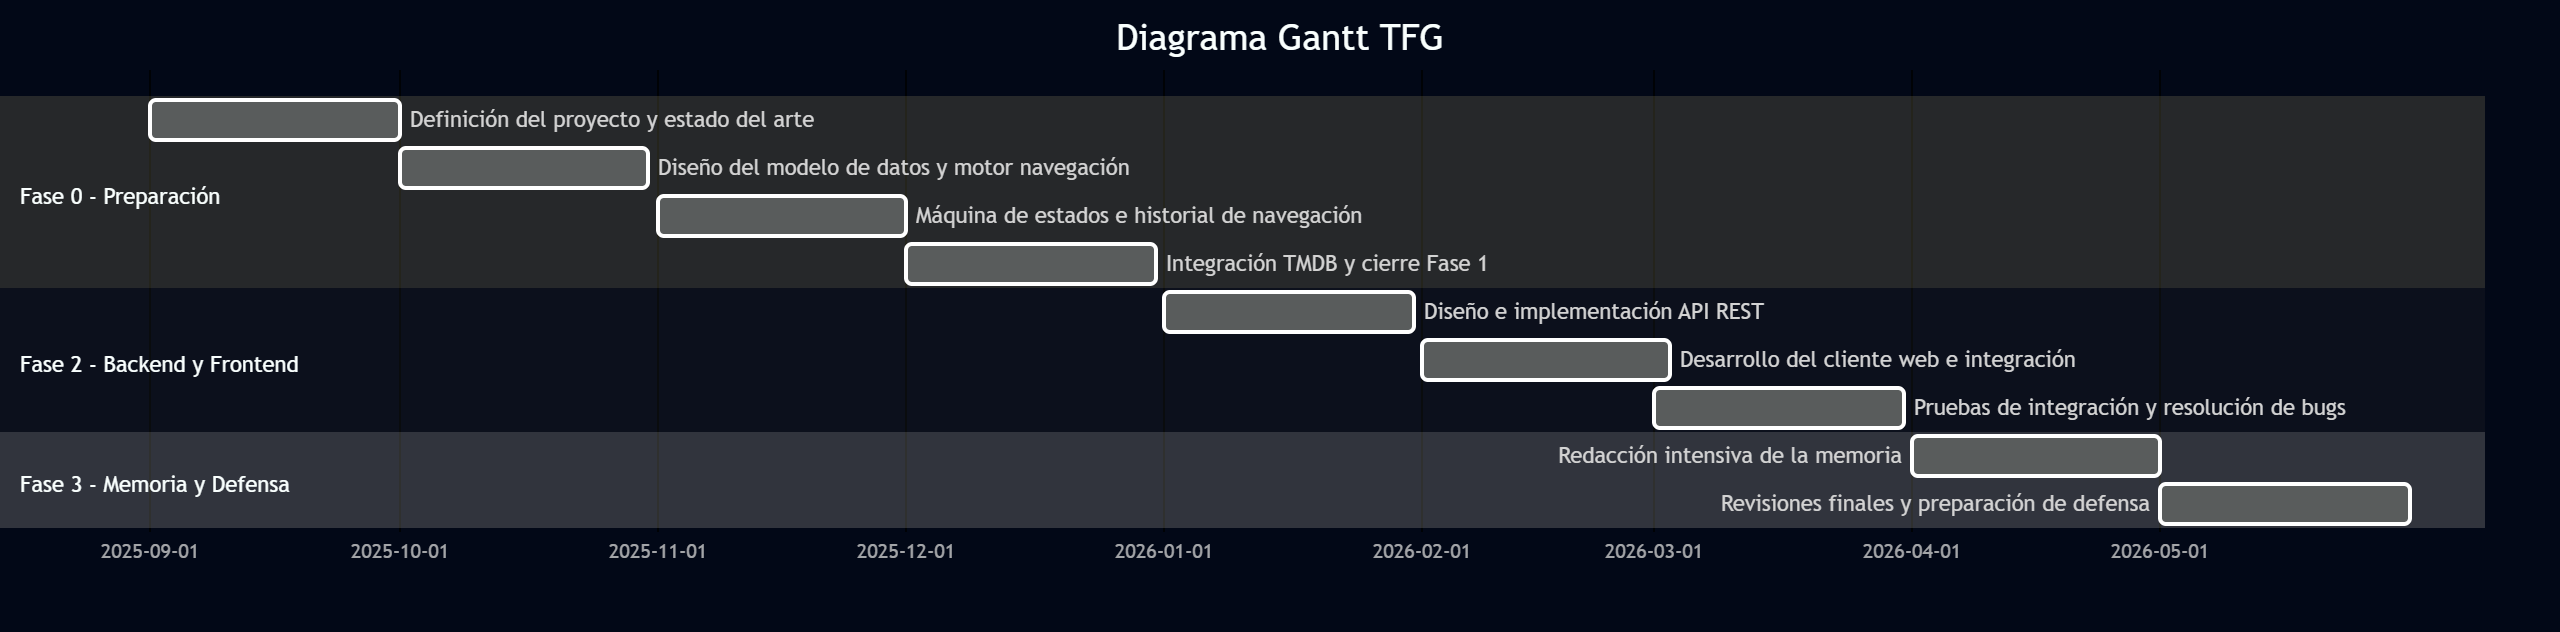
\includegraphics[width=1.2\textwidth]{Imagenes/Diagramas/Gantt.png}
}
\caption{Diagrama Gantt TFG}
\label{fig:diagramaGantt}
\end{figure}

\section{Organización de la memoria}
\label{sec:organizacionMemoria}

El resto de la memoria se estructura en cinco capítulos numerados, una sección de
\textit{Contribuciones Personales} y tres apéndices, organizados según una progresión clásica
de planteamiento, diseño, implementación, validación y cierre.

El capítulo~\ref{cap:estadoDeLaCuestion}, \textbf{Estado de la Cuestión}, sitúa el trabajo en el
marco teórico de la navegación basada en etiquetas y en los modelos de hipermedia estructurada,
y revisa los trabajos relacionados con los que el sistema dialoga de manera más directa, en
particular la plataforma Clavy y las propuestas recientes basadas en grandes modelos del
lenguaje. Aquí se identifica qué decisiones del proyecto son herederas de aportaciones previas
y cuáles toman deliberadamente otro camino.

El capítulo~\ref{cap:arquitecturaMetodologia}, \textbf{Arquitectura y Metodología}, presenta
la organización del proceso de ingeniería del software seguido, con la adopción de \textbf{Scrum}
adaptada a un equipo reducido, y la arquitectura global del sistema en términos de capas, módulos
y contratos entre ellos. Cierra con la descripción de la capa de persistencia y de la estrategia
de acceso a datos sobre PostgreSQL.

El capítulo~\ref{cap:desarrolloImplementacion}, \textbf{Desarrollo e Implementación}, profundiza
en los componentes concretos que materializan las primitivas del motor. Recorre, por este orden,
el modelo de datos relacional, la representación del contexto de exploración (la máquina de
estados), el filtrado clásico y relacional, la navegación transversal mediante \textit{links},
las operaciones de conjuntos sobre los resultados parciales, el desarrollo del cliente web y los
obstáculos encontrados junto con las soluciones aplicadas.

El capítulo~\ref{cap:pruebasValidacion}, \textbf{Pruebas y Validación}, recoge la validación del
sistema desde dos perspectivas complementarias. La primera, funcional, sobre los dos dominios de
prueba seleccionados (TMDB y DBLP). La segunda, que ocupa el grueso del capítulo, es la
evaluación formal de usabilidad con usuarios externos siguiendo un protocolo de
\textit{think-aloud} acompañado de los cuestionarios SUS y SEQ. Se reportan los resultados
cuantitativos, los hallazgos cualitativos, las iteraciones de interfaz derivadas y los casos de
uso validados, y se cierra con la enumeración explícita de las limitaciones del estudio.

El capítulo~\ref{cap:conclusiones}, \textbf{Conclusiones y Trabajo Futuro}, sintetiza el grado de
cumplimiento de los objetivos planteados en este capítulo, reconoce los límites del sistema
entregado y enumera las cinco líneas de continuación naturales identificadas a partir del estado
del trabajo. La sección de \textit{Contribuciones Personales} que sigue al capítulo de
Conclusiones documenta el reparto del trabajo entre los dos autores.

Tres apéndices completan la memoria. El apéndice~\ref{Appendix:Guion} reproduce el guion completo
de la evaluación de usabilidad, de manera que el estudio pueda replicarse sin modificaciones por
terceros. El apéndice~\ref{Appendix:integracion} describe la integración e ingesta de las fuentes
de datos externas (TMDB y DBLP), con detalle de los \textit{scripts} de captura y transformación.
El apéndice~\ref{Appendix:despliegue} documenta el despliegue del sistema sobre contenedores y
recoge las decisiones operativas que permiten reproducir el entorno de ejecución. Las versiones
en inglés de la Introducción y de las Conclusiones, exigidas por la normativa del grado, se
incluyen como capítulos no numerados al final de la memoria.